\documentclass[12pt,letterpaper]{article}

\usepackage[utf8]{inputenc}
\usepackage[spanish]{babel}
\usepackage{graphicx}
\usepackage[hidelinks]{hyperref}
\usepackage{hyperref}
\usepackage[left=2cm,right=2cm,top=2.5cm,bottom=2cm]{geometry}
\usepackage{graphicx}
\usepackage{float}
\usepackage{amsmath}
\usepackage{stackrel} 
\usepackage{multicol}
\usepackage{multirow}
\usepackage{fancyhdr}
\usepackage[usenames,dvipsnames,svgnames,table]{xcolor}
\usepackage[document]{ragged2e}
\usepackage{enumerate}

\usepackage{helvet}

\renewcommand{\labelitemi}{$-$}
\renewcommand{\labelitemii}{$\cdot$}
\newcommand\tab[1][1cm]{\hspace*{#1}}

\renewcommand{\familydefault}{\sfdefault}

\definecolor{azul}{RGB}{0,0,255}

\pagestyle{fancy}
\lhead{\begin{picture}(0,0) \put(0,0){
\includegraphics[width=10mm]{./img/logo}} \end{picture}}
\chead{\hspace{1cm}\vspace{0.2cm}Laboratorio 06 - Reportes con Google Data Studio}
\rhead{}

\begin{document}
    \begin{titlepage}
        \begin{center}
            \begin{figure}[htb]
                \begin{center}
                    
\includegraphics[width=3.5cm]{./img/logo}
                \end{center}
            \end{figure}
            \vspace*{0.15in}
            \begin{Large}
                \textbf{UNIVERSIDAD PRIVADA DE TACNA}\\
            \end{Large}
            \vspace*{0.15in}
            \begin{Large}
                \textbf{FACULTAD DE INGENIERÍA} \\
            \end{Large}
            \vspace*{0.1in}
            \begin{Large}
                \textbf{Escuela Profesional de Ingeniería de Sistemas} \\
            \end{Large}
            \vspace*{0.3in}
            \begin{Large}
                \textbf{Laboratorio 06}\\
                \textbf{``Reportes con Google Data Studio"}\\
            \end{Large}
            \vspace*{0.2in}
            \begin{Large}
                \textbf{CURSO:} \\
            \end{Large}
            \vspace*{0.1in}
            \begin{large}
                Inteligencia de Negocios\\
            \end{large}
            \vspace*{0.2in}
            \begin{Large}
                \textbf{DOCENTE:} \\
            \end{Large}
            \vspace*{0.1in}
            \begin{large}
                Mag. Patrick Jose Cuadros Quiroga\\
            \end{large}
            \vspace*{0.3in}
            \begin{large}
                \textbf{ALUMNO:} \\
                \begin{flushleft}
                    Lipa Calabilla, Abraham  		\hfill	(2019064039) \\
                \end{flushleft}
            \end{large}
            \vspace*{1.3in}
            \begin{large}
                Tacna - Perú\\
            \end{large}
            \vspace*{0.1in}
            \begin{large}
                2022\\
            \end{large}
        \end{center}
    \end{titlepage}
    \include{Secciones/articulo}
    \newpage
    \tableofcontents
    \justify
    \newpage
    \begin{LARGE}
        \begin{center}
            \textbf{REPORTES CON GOOGLE DATA STUDIO} \\
        \end{center}
    \end{LARGE}
    \section{OBJETIVOS}
    \begin{itemize}
        \item Crear reportes on Google Data Studio.
    \end{itemize}

    \section{REQUERIMIENTOS}
    \begin{itemize}
        \item Conocimientos\\
        Para el desarrollo de esta práctica se requerirá de los siguientes conocimientos básicos:
        \begin{itemize} 
            \item Conocimientos básicos de uso de Google Data Studio.
        \end{itemize}
        \item Hardware
        \begin{itemize}
            \item CPU SLAT-capable feature.
            \item Al menos 4GB de RAM.
        \end{itemize}
        \item Software\\
        Así mismo se necesitan los siguientes aplicativos
        \begin{itemize}
            \item Google Data Studio (cuenta de Google requerida)
            \item Google Drive y Google Sheets
        \end{itemize}
    \end{itemize}

    \newpage
    \section{DESARROLLO}
    \subsection{Parte 1: Crear la fuente de datos}
    \begin{enumerate}[\tab 1.]
        \item Abrir \textcolor{azul}{\url{datastudio.google.com}} e iniciar sesión con su cuenta de Google\\[0.1in]
        \begin{center}
            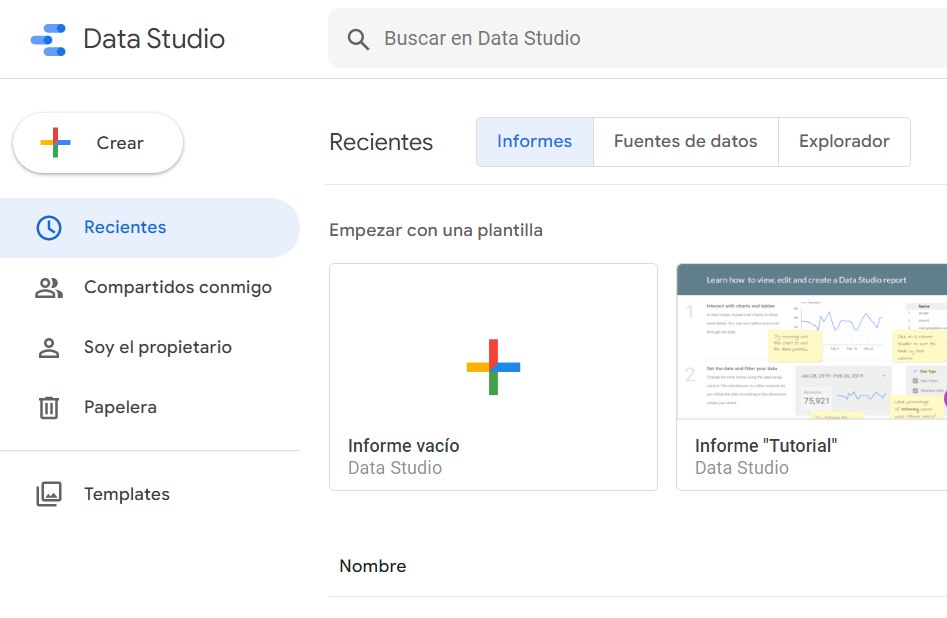
\includegraphics[width=13cm]{./img/img1.png}
        \end{center}
        \item Abrir Google Drive y crear una hoja de calculo de Google Sheet en blanco
        \item Renombrar la hoja “Covid Data”
        \item En la primera celda, escribir la formula \\
        =IMPORTHTML("https://www.worldometers.info/coronavirus/", "table",1)
        \begin{center}
            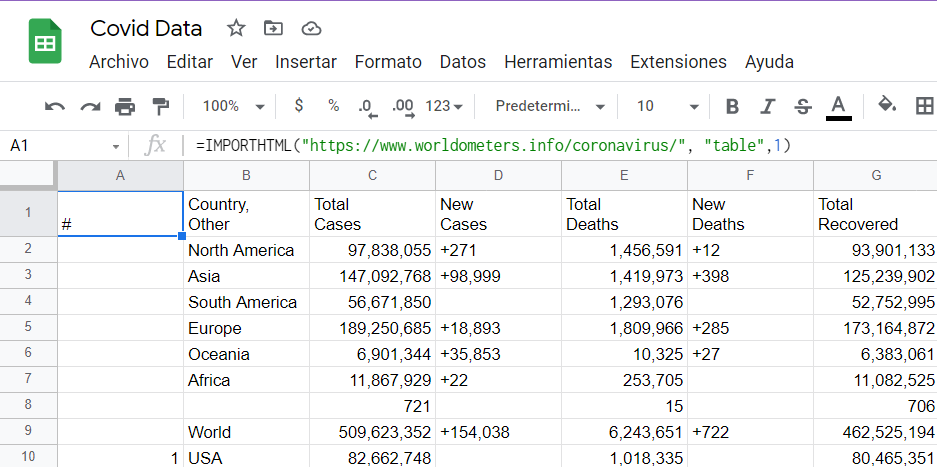
\includegraphics[width=13cm]{./img/img2.png}
        \end{center}
    \end{enumerate}

    \subsection{Parte 2: Crear el Origen de Datos}
    \begin{enumerate}[\tab 1.]
        \item En Data Studio, haga click en el botón Crear y selecciones Informes
        \begin{center}
            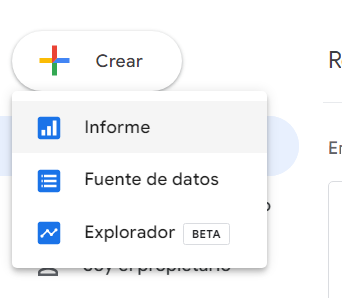
\includegraphics[width=6cm]{./img/img3.png}
        \end{center}
        \item Completar las opciones de primera vez
        \begin{center}
            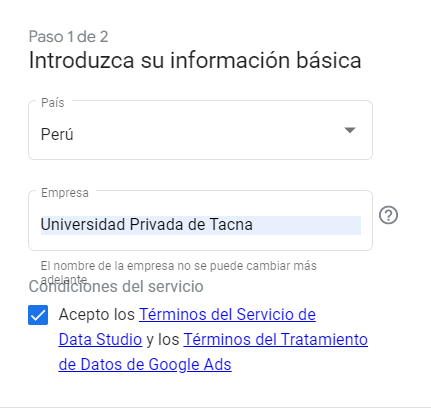
\includegraphics[width=6cm]{./img/img4.png}
        \end{center}
        \item Seleccionar el conector Google Sheet y añadir la hoja “Covid Data”
        \begin{center}
            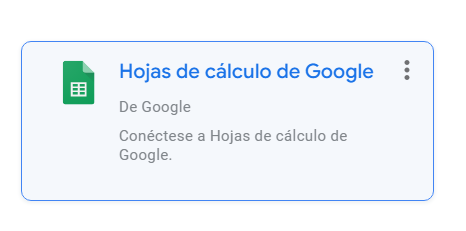
\includegraphics[width=6cm]{./img/img5.png}
        \end{center}
        \item Ocultar las filas no deseadas en la hoja
        \begin{center}
            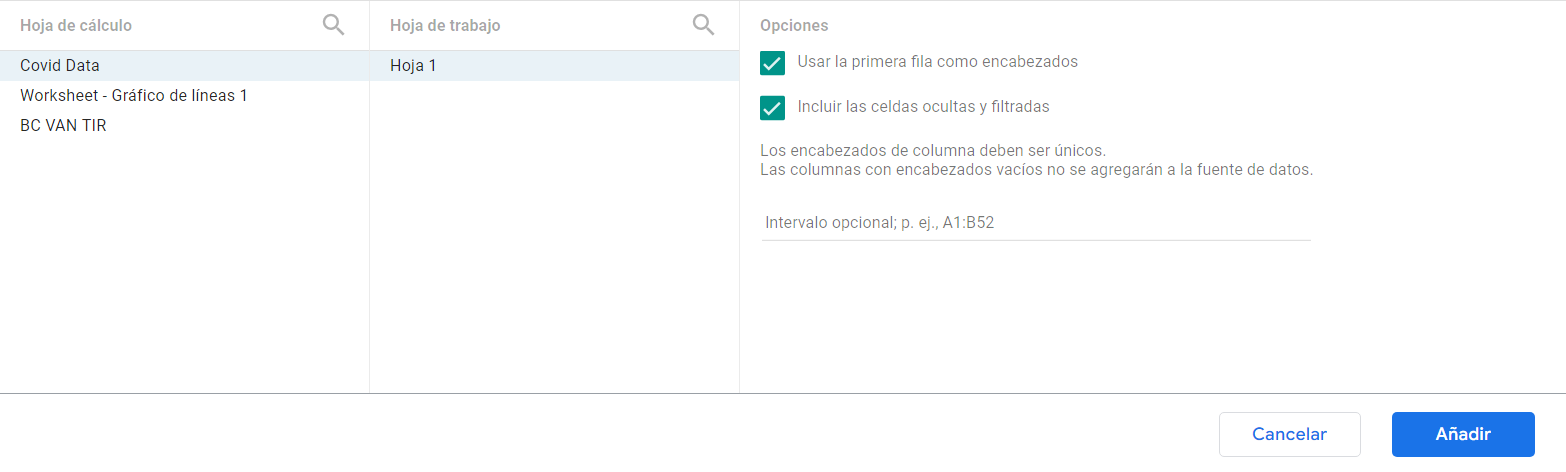
\includegraphics[width=13cm]{./img/img6.png}
        \end{center}
        \item Desmarcar la opción "Incluir celdas ocultas y filtradas” y luego hacer click en Añadir reporte o Conectar
        \begin{center}
            
\includegraphics[width=5cm]{./img/img7.png}
        \end{center}
    \end{enumerate}

    \subsection{Parte 3: Añadir campos al origen de datos}
    \begin{enumerate}[\tab 1.]
        \item En el menú Recurso, abrir “Gestión de las fuentes de datos añadidas” y click en Editar
        \begin{center}
            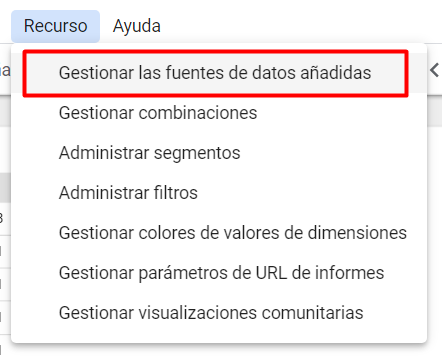
\includegraphics[width=6cm]{./img/img8.png}
        \end{center}
        \begin{center}
            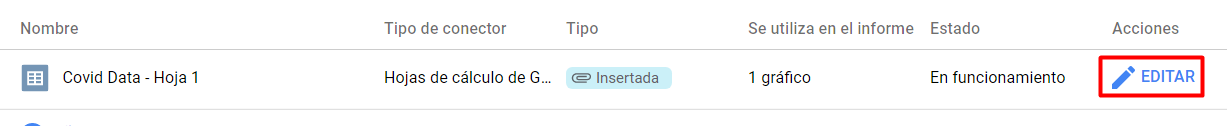
\includegraphics[width=13cm]{./img/img9.png}
        \end{center}
        \item Verificar los datos y sus tipos de datos
        \item Deshabilitar el campo Conteo o cantidad de registros o filas
        \begin{center}
            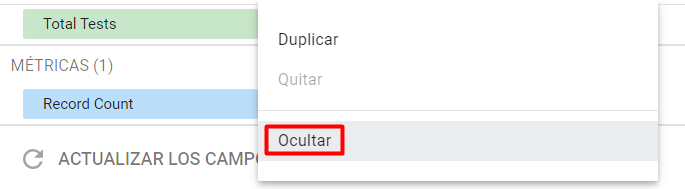
\includegraphics[width=6cm]{./img/img10.png}
        \end{center}
        \begin{center}
            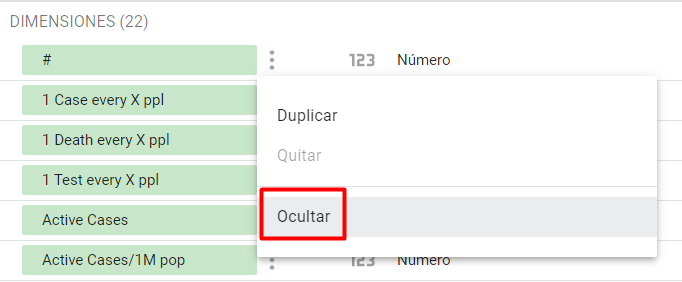
\includegraphics[width=6cm]{./img/img11.png}
        \end{center}
        \item Crear dos nuevos Campos
        \begin{center}
            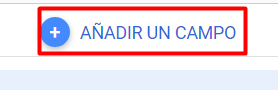
\includegraphics[width=5cm]{./img/img12.png}
        \end{center}
        \begin{enumerate}
            \item Casos mundiales. Formula SUM(Total Cases)
            \begin{center}
                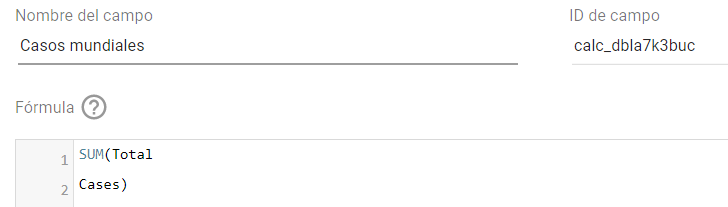
\includegraphics[width=13cm]{./img/img13.png}
            \end{center}
            \item Tasa de Mortalidad. Formula (Total deaths/ Total cases)
            \begin{center}
                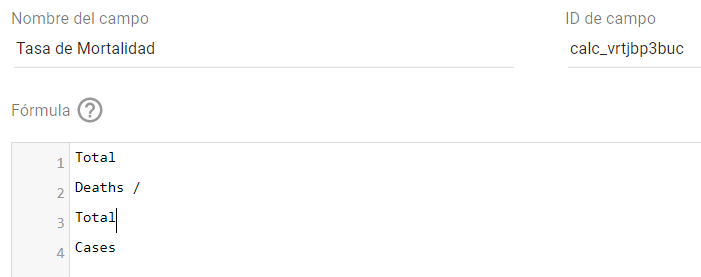
\includegraphics[width=13cm]{./img/img14.png}
            \end{center}
        \end{enumerate}
    \end{enumerate}

    \subsection{Paso 4: Crear Diferentes Dashboards}
    \begin{enumerate}[\tab 1.]
        \item Total de casos por continente
        \begin{center}
            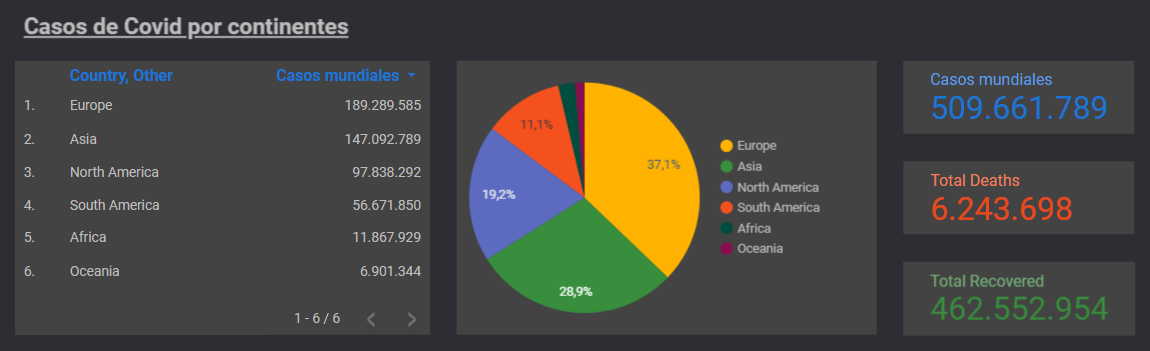
\includegraphics[width=13cm]{./img/img15.png}
        \end{center}
        \item Total de casos en el mapa
        \begin{center}
            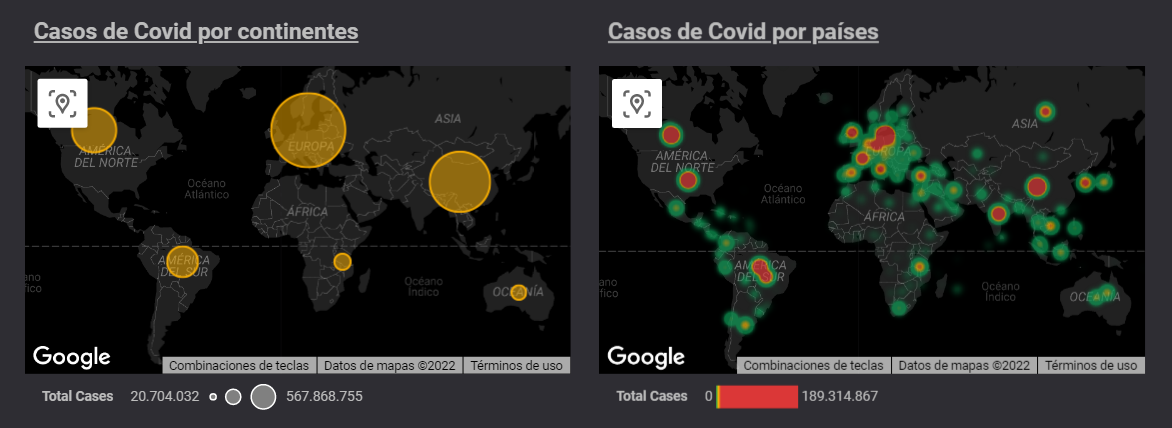
\includegraphics[width=13cm]{./img/img16.png}
        \end{center}
    \end{enumerate}

    \newpage
    \section{CONCLUSIONES}
    \begin{itemize}
        \item Se logró utilizar los servicios de Google para realizar un análisis de los datos relacionados al COVID-19. Se pudo crear los datos e importarlos desde Google Sheets a Google Data Studio. Así mismo, se pudo manipular los datos para finalmente poder visualizarlos de manera intuitiva y agradable al usuario.
    \end{itemize}
\end{document}